\documentclass{article}
\usepackage[backend=biber, style=numeric, citestyle=numeric]{biblatex}
\addbibresource{bibliography.bib}
\usepackage{graphicx}
\usepackage{amsmath, bm, amssymb}
\usepackage{titlesec}
\usepackage{geometry}
\usepackage{fancyhdr}
\usepackage{xcolor}
\usepackage{algorithm}
\usepackage{algpseudocode}
\usepackage{hyperref}
\usepackage{caption}
\usepackage{subcaption}
\usepackage{color}
\definecolor{darkred}{rgb}{0.6,0.0,0.0}
\definecolor{darkgreen}{rgb}{0,0.50,0}
\definecolor{lightblue}{rgb}{0.0,0.42,0.91}
\definecolor{orange}{rgb}{0.99,0.48,0.13}
\definecolor{grass}{rgb}{0.18,0.80,0.18}
\definecolor{pink}{rgb}{0.97,0.15,0.45}

% listings
\usepackage{listings}

% General Setting of listings
\lstset{
  aboveskip=1em,
  breaklines=true,
  abovecaptionskip=-6pt,
  captionpos=b,
  escapeinside={\%*}{*)},
  frame=single,
  numbers=left,
  numbersep=15pt,
  numberstyle=\tiny,
}
% 0. Basic Color Theme
\lstdefinestyle{colored}{ %
  basicstyle=\ttfamily,
  backgroundcolor=\color{white},
  commentstyle=\color{green}\itshape,
  keywordstyle=\color{blue}\bfseries\itshape,
  stringstyle=\color{red},
}
% 1. General Python Keywords List
\lstdefinelanguage{PythonPlus}[]{Python}{
  morekeywords=[1]{,as,assert,nonlocal,with,yield,self,True,False,None,} % Python builtin
  morekeywords=[2]{,__init__,__add__,__mul__,__div__,__sub__,__call__,__getitem__,__setitem__,__eq__,__ne__,__nonzero__,__rmul__,__radd__,__repr__,__str__,__get__,__truediv__,__pow__,__name__,__future__,__all__,}, % magic methods
  morekeywords=[3]{,object,type,isinstance,copy,deepcopy,zip,enumerate,reversed,list,set,len,dict,tuple,range,xrange,append,execfile,real,imag,reduce,str,repr,}, % common functions
  morekeywords=[4]{,Exception,NameError,IndexError,SyntaxError,TypeError,ValueError,OverflowError,ZeroDivisionError,}, % errors
  morekeywords=[5]{,ode,fsolve,sqrt,exp,sin,cos,arctan,arctan2,arccos,pi, array,norm,solve,dot,arange,isscalar,max,sum,flatten,shape,reshape,find,any,all,abs,plot,linspace,legend,quad,polyval,polyfit,hstack,concatenate,vstack,column_stack,empty,zeros,ones,rand,vander,grid,pcolor,eig,eigs,eigvals,svd,qr,tan,det,logspace,roll,min,mean,cumsum,cumprod,diff,vectorize,lstsq,cla,eye,xlabel,ylabel,squeeze,}, % numpy / math
}
% 2. New Language based on Python
\lstdefinelanguage{PyBrIM}[]{PythonPlus}{
  emph={d,E,a,Fc28,Fy,Fu,D,des,supplier,Material,Rectangle,PyElmt},
}
% 3. Extended theme
\lstdefinestyle{colorEX}{
  basicstyle=\ttfamily,
  backgroundcolor=\color{white},
  commentstyle=\color{darkgreen}\slshape,
  keywordstyle=\color{blue}\bfseries\itshape,
  keywordstyle=[2]\color{blue}\bfseries,
  keywordstyle=[3]\color{grass},
  keywordstyle=[4]\color{red},
  keywordstyle=[5]\color{orange},
  stringstyle=\color{darkred},
  emphstyle=\color{pink}\underbar,
}





\geometry{left=1in, right=1in, top=1in, bottom=1in}

\definecolor{titlecolor}{RGB}{0, 0, 48}

\titleformat{\section}[block]{\normalfont\Large\bfseries\color{titlecolor}}{\thesection}{1em}{}
\titleformat{\subsection}[block]{\normalfont\large\bfseries\color{titlecolor}}{\thesubsection}{1em}{}

\pagestyle{fancy}
\fancyhf{}
\lhead{\scriptsize EEC 289A Assignment 2 Report}
\rhead{}
\cfoot{\thepage}

\begin{document}

\noindent
\textbf{\large EEC 289A Assignment 2 Report} \\
\textbf{\small Chenye Yang, Hanchu Zhou, Haodong Liang, Yibo Ma}



\section{Introduction}

Texture synthesis has been an active research topic in computer vision both as a way to verify texture analysis methods, as well as in its own right. Potential applications
of a successful texture synthesis algorithm are broad, including occlusion fill-in, lossy image and video compression, foreground removal, etc. 

This project seeks to reproduce and expand upon the work by Efros \& Leung (1999) on non-parametric texture synthesis~\cite{790383}. Originally, this method was groundbreaking for its ability to synthesize new texture fields that maintain the visual characteristics of a given sample texture. Our primary objective is to apply this technique to the textures assigned in the class, exploring both the effectiveness and the limitations of the method in replicating and scaling up these specific patterns.

In addition to replication, this project will extend the methodology to other images and contexts of interest. Particularly, we aim to test the feasibility of applying texture synthesis techniques to generate MNIST digits and a galaxy picture\footnote{Galaxy starry night sky background, free public domain CC0 photo. \url{https://www.rawpixel.com/image/5924106/photo-image-public-domain-stars-galaxy}}, which present a unique challenge in scaling the approach to handle more complex and structured data.

% Moreover, we delve into some theoretical questions that arise from the practice of generative modeling. In summary, this report outlines our approaches, experiments, and tries to answer the following questions in the slides:
% \begin{enumerate}
%     \item Scale up non-parametric texture synthesis?
%     \item Why are generative models assign higher probability to something it has not been trained on?
%     \item Can we use the state-of-the-art open-sourced large language models to re-estimate the upper bound of the conditional entropy of text, like Shannon has done in 1951?
%     \item Can you learn the words from text with dictionary learning?
% \end{enumerate}




\section{Algorithm Overview}
This algorithm synthesizes texture by expanding pixel by pixel from an initial seed point. It uses a single pixel, $p$, as the synthesis unit to capture as much high-frequency information as possible. All previously synthesized pixels within a square window surrounding $p$ (with weights to highlight local structures) serve as the context. To continue the synthesis, probability tables for the distribution of $p$ are needed for all possible contexts. However, while these tables are typically manageable in size for textual data, constructing them explicitly for textures is impractical. An approximation might be achieved using various clustering techniques, but we opt not to construct a model at all. Instead, each new context queries the sample image, and the distribution of $p$ is created as a histogram of all possible values found in the sample image, as demonstrated in Figure 1. This non-parametric sampling method, though simple, is highly effective at capturing statistical processes for which an adequate model has not yet been developed.

\begin{figure}[htbp!]
    \centering
    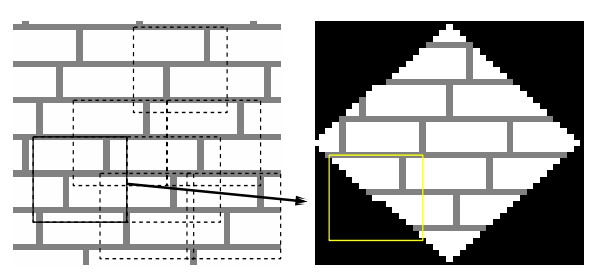
\includegraphics[scale=0.8]{Fig1.jpg}
    \caption{Algorithm Overview}
    \label{fig:enter-label}
\end{figure}

In this work, the texture is modeled as a Markov Random Field (MRF). That is, we assume that the probability distribution of brightness values for a pixel, given the brightness values of its spatial neighborhood, is independent of the rest of the image. The neighborhood of a pixel is modeled as a square window around that pixel. The size of the window is a free parameter that specifies how stochastic the user believes this texture to be. More specifically, if the texture is presumed to be mainly regular at high spatial frequencies and mainly stochastic at low spatial frequencies, the size of the window should be on the scale of the biggest regular feature. 

\subsection{Synthesizing one pixel}
Let \( I \) be an image that is being synthesized from a texture sample image \( I_{\text{smp}} \subset I_{\text{real}} \) where \( I_{\text{real}} \) is the real infinite texture. Let \( p \in I \) be a pixel and let \( \omega(p) \subset I \) be a square image patch of width \( w \) centered at \( p \). Let \( d_{\text{perc}}(\omega_1, \omega_2) \) denote some perceptual distance between two patches. Assume that all pixels in \( I \) except for \( p \) are known. To synthesize the value of \( p \) we first construct an approximation to the conditional probability distribution \( P(p \mid \omega(p)) \) and then sample from it.

Based on our MRF model, we assume that \( p \) is independent of \( I \setminus \omega(p) \) given \( \omega(p) \). Define a set
\[
\Omega(p) = \{\omega' \subset I_{\text{real}} : d_{\text{perc}}(\omega_0, \omega(p)) = 0\}
\]
containing all occurrences of \( \omega(p) \) in \( I_{\text{real}} \), then the conditional PDF of \( p \) can be estimated with a histogram of all center pixel values in \( \Omega(p) \). Unfortunately, we are only given \( I_{\text{smp}}, \) a finite sample from \( I_{\text{real}}, \) which means there might not be any matches for \( \omega(p) \) in \( I_{\text{smp}} \). Thus, we must use a heuristic which will let us find a plausible \( \Omega'(p) \approx \Omega(p) \) to sample from. In our implementation, a variation of the k-Nearest Neighbors technique is used: the closest match \( \omega'_{\text{best}} = \arg\min_{\omega} d_{\text{perc}}(\omega(p), \omega) \in I_{\text{smp}} \) is found, and all image patches \( \omega_0 \) with \( d_{\text{perc}}(\omega'_{\text{best}}, \omega') < \epsilon \) are included in \( \Omega' \), where \( \epsilon \) is a threshold. The center pixel values of patches in \( \Omega' \) give us a histogram for \( p \), which can then be sampled, either uniformly or weighted by \( d_{\text{perc}} \).

Now it only remains to find a suitable \( d_{\text{perc}} \). One choice is a normalized sum of squared differences metric \( d_{\text{SSD}} \). However, this metric gives the same weight to any mismatched pixel, whether near the center or at the edge of the window. Since we would like to preserve the local structure of the texture as much as possible, the error for nearby pixels should be greater than for pixels far away. To achieve this effect we set \( d_{\text{perc}} = d_{\text{SSD}} \cdot G \) where \( G \) is a two-dimensional Gaussian kernel.


\subsection{Synthesizing texture}
In the previous section, we discussed a method of synthesizing a pixel when its neighborhood pixels are already known. Unfortunately, this method cannot be used for synthesizing the entire texture or even for hole-filling (unless the hole is just one pixel) since for any pixel the values of only some of its neighborhood pixels will be known. The correct solution would be to consider the joint probability of all pixels together, but this is intractable for images of realistic size.

Instead, a Shannon-inspired heuristic is proposed, where the texture is grown in layers outward from a 3-by-3 seed taken randomly from the sample image (in case of hole-filling, the synthesis proceeds from the edges of the hole). Now for any point \( p \) to be synthesized only some of the pixel values in \( \omega(p) \) are known (i.e., have already been synthesized). Thus, the pixel synthesis algorithm must be modified to handle unknown neighborhood pixel values. This can be easily done by only matching on the known values in \( \omega(p) \) and normalizing the error by the total number of known pixels when computing the conditional pdf for \( p \). This heuristic does not guarantee that the pdf for \( p \) will stay valid as the rest of \( \omega(p) \) is filled in. However, it appears to be a good approximation in practice. One can also treat this as an initialization step for an iterative approach such as Gibbs sampling. However, our trials have shown that Gibbs sampling produced very little improvement for most textures. This lack of improvement indicates that the heuristic indeed provides a good approximation to the desired conditional pdf.

\section{Experiments}
\subsection{Textures}

We apply the non-parametric texture synthesis method to the following textures: the textures provided in the class, the MNIST digits, and the galaxy picture we chosen. 
The textures provided in the class have the size around $530 \times 530$, shown in Figure~\ref{fig:texture-class}.

\begin{figure}[htbp!]
    \centering
    \begin{subfigure}[b]{0.3\textwidth}
        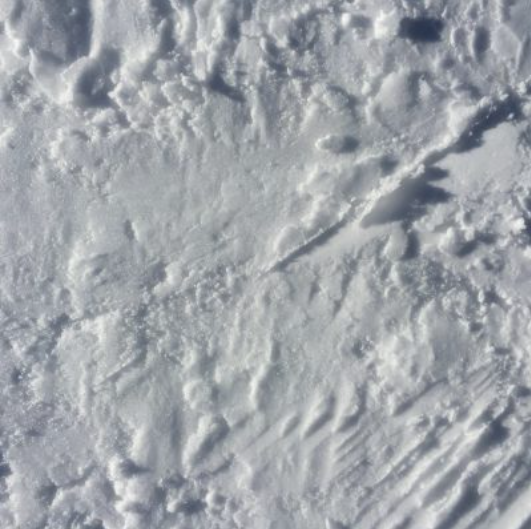
\includegraphics[width=\textwidth]{../Code/Textures/2.png}
        \caption{Texture 2}
        \label{fig:texture-2}
    \end{subfigure}
    \hfill % this will add space between the subfigures
    \begin{subfigure}[b]{0.3\textwidth}
        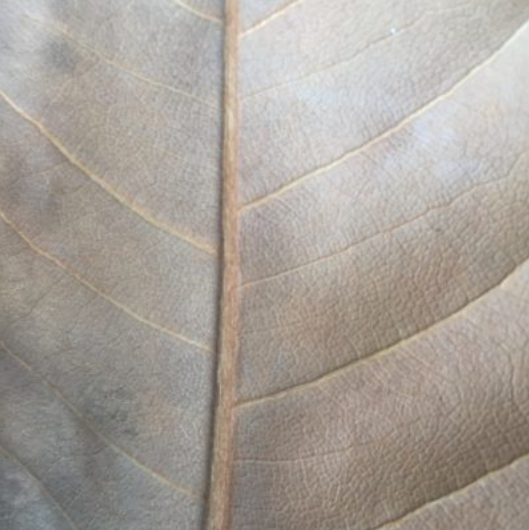
\includegraphics[width=\textwidth]{../Code/Textures/4.png}
        \caption{Texture 4}
        \label{fig:texture-4}
    \end{subfigure}
    \hfill % this will add space between the subfigures
    \begin{subfigure}[b]{0.3\textwidth}
        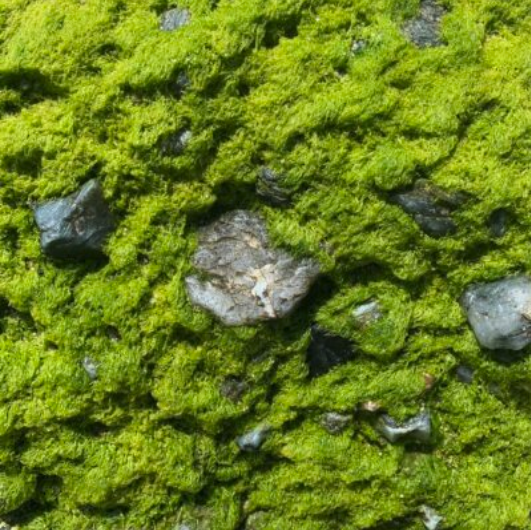
\includegraphics[width=\textwidth]{../Code/Textures/9.png}
        \caption{Texture 9}
        \label{fig:texture-9}
    \end{subfigure}
    \caption{Texture: provided in the class}
    \label{fig:texture-class}
\end{figure}

For the MNIST digits, we load the MNIST dataset ($28 \times 28$ handwritten digits)\footnote{Downloaded from \url{https://git-disl.github.io/GTDLBench/datasets/mnist_datasets/}}, including 60000 training images and 10000 testing images. 
We randomly select $20 \times 20$ images from the training set as the sample texture of size $560 \times 560$, shown in Figure~\ref{fig:texture-mnist}.

\begin{figure}[H]
    \centering
    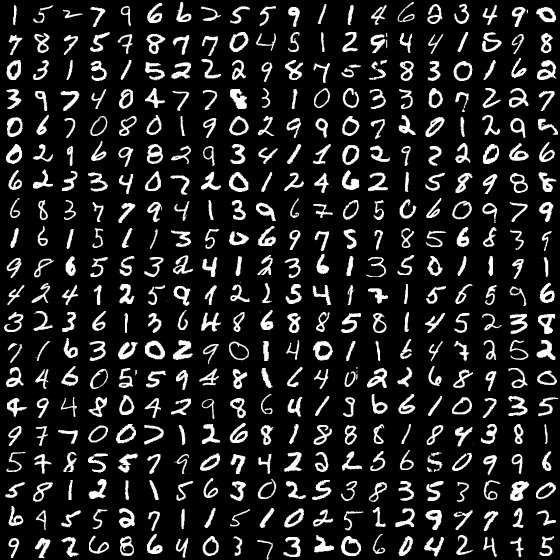
\includegraphics[scale=0.4]{../Code/Textures/mnist.png}
    \caption{Texture: MNIST digits}
    \label{fig:texture-mnist}
\end{figure}

For the galaxy picture, we load the galaxy picture ($800 \times 585$), shown in Figure~\ref{fig:texture-galaxy}.
\begin{figure}[H]
    \centering
    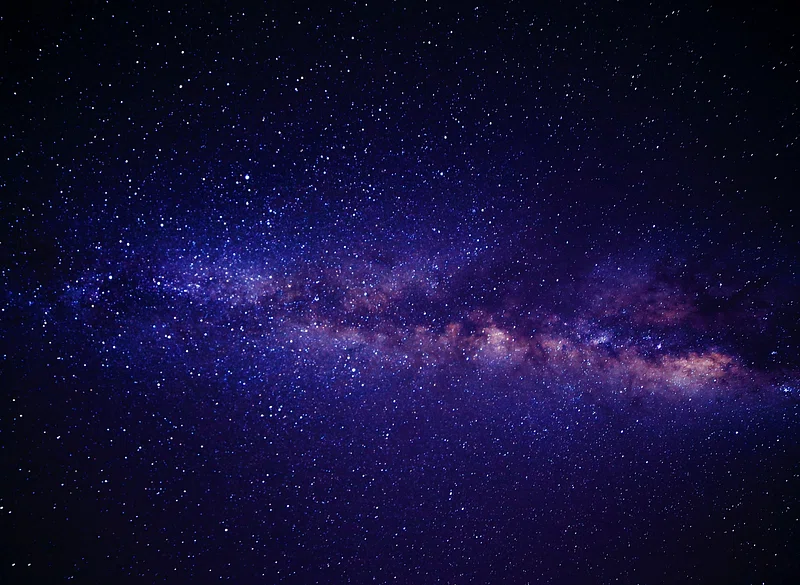
\includegraphics[width=0.4\textwidth]{../Code/Textures/galaxy.png}
    \caption{Texture: galaxy picture}
    \label{fig:texture-galaxy}
\end{figure}

\subsection{Non-parametric Texture Synthesis}

The algorithm proposed by Efros \& Leung (1999)~\cite{790383}, Algorithm~\ref{alg:texture-synthesis}, synthesizes texture by modeling the image as a Markov Random Field (MRF) where each pixel's value is dependent only on the values in its immediate neighborhood. 
The texture synthesis process grows the new image pixel by pixel from an initial seed based on this model. Here are some important features about the algorithm:
\begin{itemize}
  \item {Non-parametric approach:} The algorithm does not build an explicit model but estimates pixel distributions dynamically from the sample image.
  \item {Control over randomness:} The size of the neighborhood window can be adjusted to control the randomness of the texture, affecting how structured or stochastic the synthesized texture appears.
  \item {Efficiency:} A variation of the k Nearest Neighbors technique is employed to find matching neighborhoods quickly.
  \item {Local structure preservation:} Emphasis on maintaining the local structure of the texture to ensure visual continuity and realism in the synthesized image.
\end{itemize}

\begin{algorithm}
    \caption{Texture Synthesis by Non-parametric Sampling}\label{alg:texture-synthesis}
    \begin{algorithmic}[1]
    
    \State Initialize with a small seed taken randomly from the sample image $I_{\text{smp}}$.
    
    \While{there are unsynthesized pixels in the image $I$}
        \State Select an unsynthesized pixel $p$ in $I$.
        \State Define the neighborhood $N(p)$ of $p$ as a square window centered at $p$.
        
        \State Find all neighborhoods in $I_{\text{smp}}$ that are similar to $N(p)$ using a perceptual distance metric $d_{\text{perc}}$.
        \State Construct a histogram of pixel values from these similar neighborhoods to approximate the conditional probability distribution $P(p|N(p))$.
        \State Sample from this distribution to set the value of $p$.
    \EndWhile
    
    \end{algorithmic}
\end{algorithm}

\subsection{Parallelization: Multi-core Processing}

To speed up the texture synthesis process, we parallelize the algorithm by dividing the image into blocks and synthesizing each block independently, given that the processing of each pixel (and its surrounding window) is somewhat independent.
We use the Python \texttt{multiprocessing} library to create a pool of worker processes that can work on different blocks concurrently:
\begin{itemize}
    \item {Split the work:} Distribute the processing of each pixel to different CPU cores. This can be done by creating a list of tasks where each task contains the information needed to process a pixel.
    \item {Process pool:} Use a multiprocessing pool to process these tasks concurrently.
    \item {Result collection:} Collect the results from each task and update the main data structures accordingly.
\end{itemize}
With this parallelization strategy, we can achieve a significant speedup (depending on hardware, around $8\times$) in the texture synthesis process.

\section{Results}
\subsection{Texture Synthesis}
In this section, we present the results of applying the non-parametric texture synthesis method to the textures described in the previous section.
The patch size is set to $11 \times 11$ for all the textures, and the resolution is set to $1000\times 1000$ for all synthesized pictures.
The synthesized textures are shown in Figure~\ref{fig:synthesis-2} - \ref{fig:synthesis-galaxy}.

\begin{figure}[H]
    \centering
    \begin{subfigure}[b]{0.49\textwidth}
        \centering
        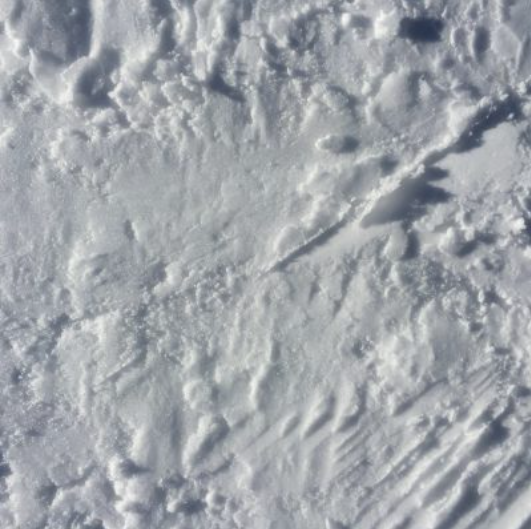
\includegraphics[width=0.5\textwidth]{../Code/Textures/2.png}
        \caption{Texture 2}
        \label{fig:original-2}
    \end{subfigure}
    \hfill % this will add space between the subfigures
    \begin{subfigure}[b]{0.49\textwidth}
        \centering
        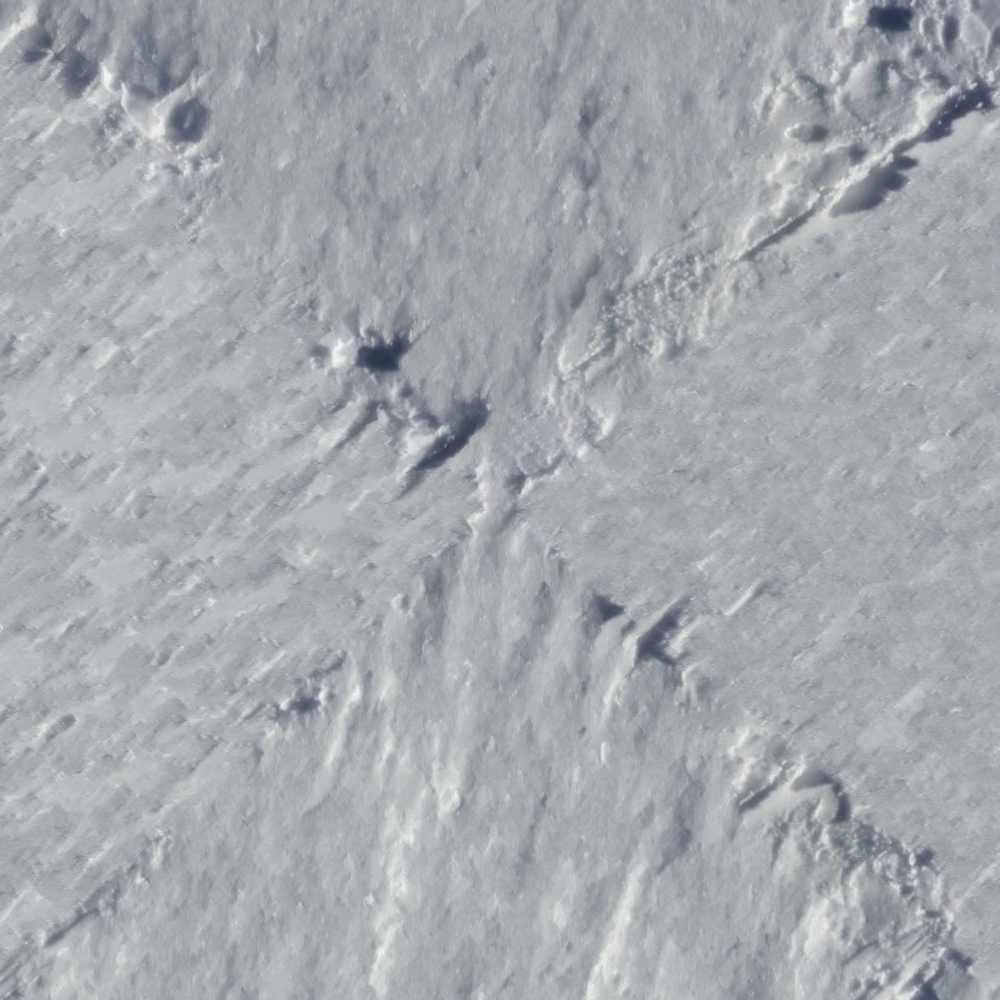
\includegraphics[width=0.7\textwidth]{../Result/2.png}
        \caption{Synthesized Texture 2}
        \label{fig:synthesized-2}
    \end{subfigure}
    \caption{Synthesis of Texture 2}
    \label{fig:synthesis-2}
\end{figure}

\begin{figure}[H]
    \centering
    \begin{subfigure}[b]{0.49\textwidth}
        \centering
        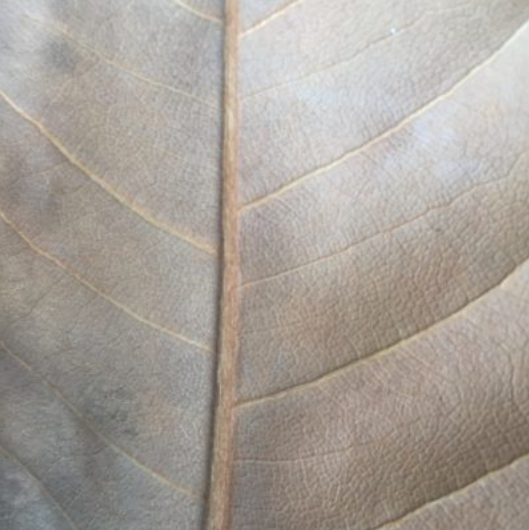
\includegraphics[width=0.5\textwidth]{../Code/Textures/4.png}
        \caption{Texture 4}
        \label{fig:original-4}
    \end{subfigure}
    \hfill % this will add space between the subfigures
    \begin{subfigure}[b]{0.49\textwidth}
        \centering
        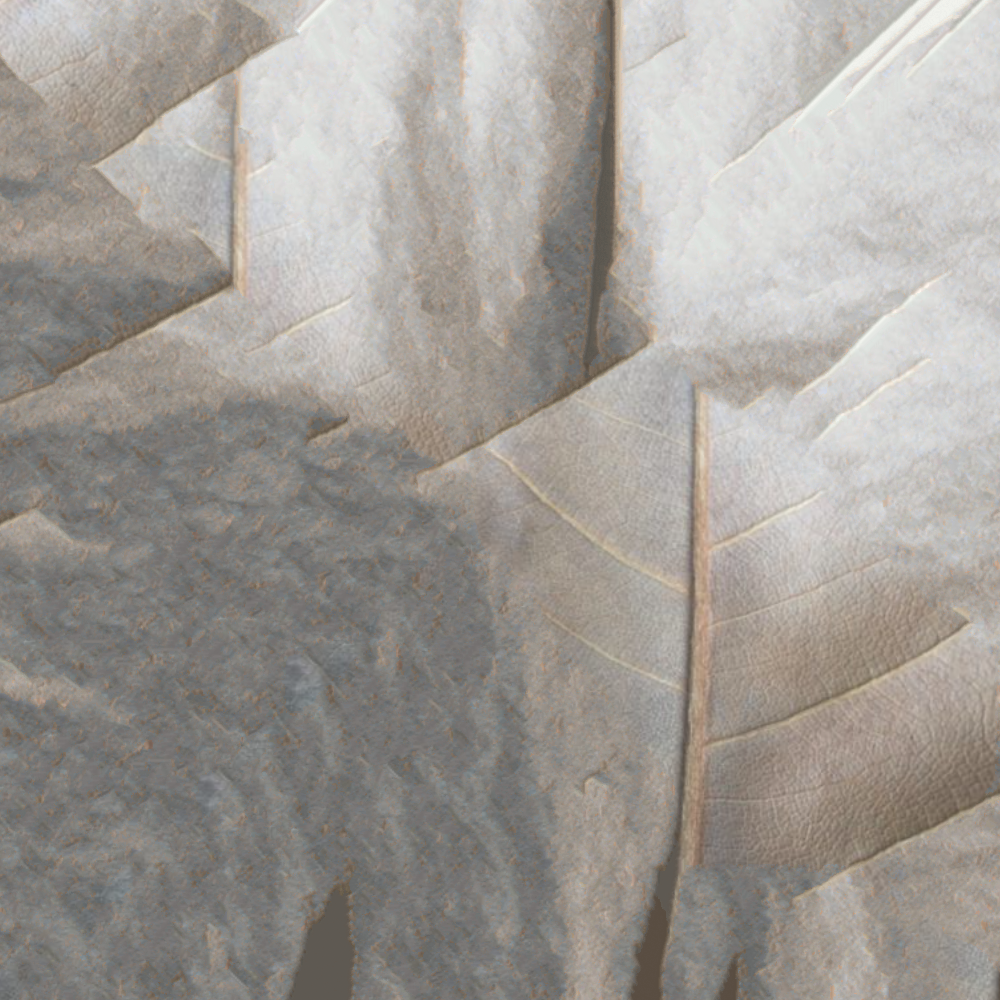
\includegraphics[width=0.7\textwidth]{../Result/4.png}
        \caption{Synthesized Texture 4}
        \label{fig:synthesized-4}
    \end{subfigure}
    \caption{Synthesis of Texture 4}
    \label{fig:synthesis-4}
\end{figure}

\begin{figure}[H]
    \centering
    \begin{subfigure}[b]{0.49\textwidth}
        \centering
        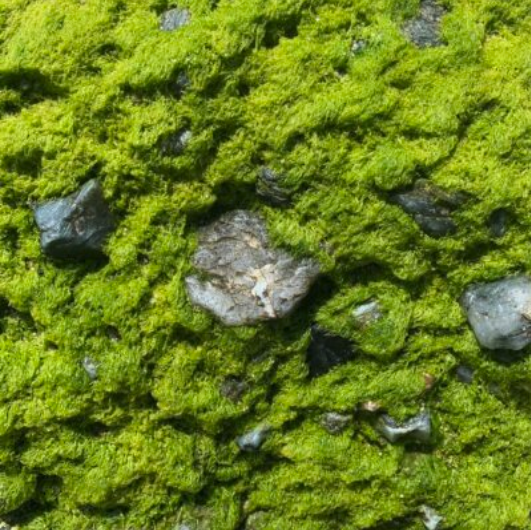
\includegraphics[width=0.5\textwidth]{../Code/Textures/9.png}
        \caption{Texture 9}
        \label{fig:original-9}
    \end{subfigure}
    \hfill % this will add space between the subfigures
    \begin{subfigure}[b]{0.49\textwidth}
        \centering
        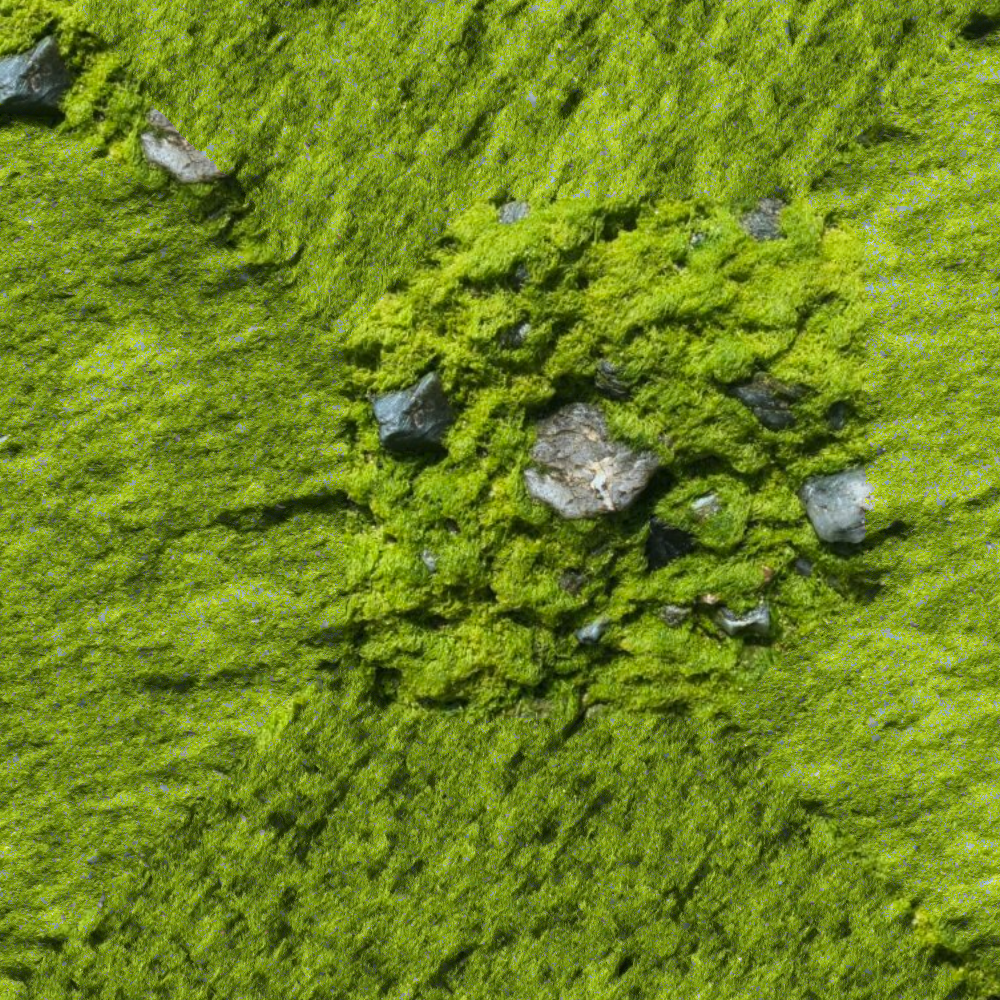
\includegraphics[width=0.7\textwidth]{../Result/9.png}
        \caption{Synthesized Texture 9}
        \label{fig:synthesized-9}
    \end{subfigure}
    \caption{Synthesis of Texture 9}
    \label{fig:synthesis-9}
\end{figure}

\begin{figure}[H]
    \centering
    \begin{subfigure}[b]{0.49\textwidth}
        \centering
        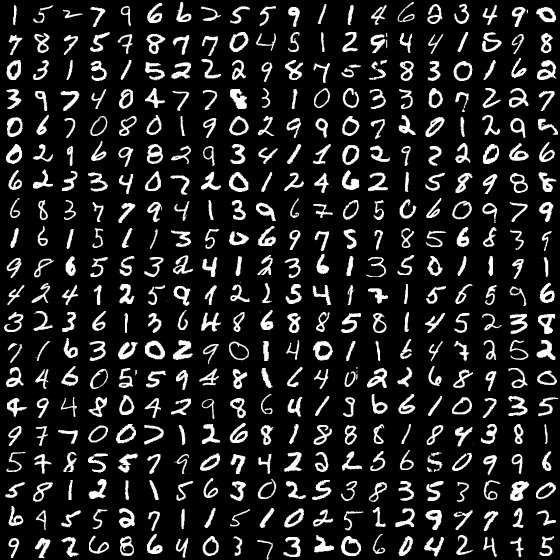
\includegraphics[width=0.5\textwidth]{../Code/Textures/mnist.png}
        \caption{MNIST Digits}
        \label{fig:original-mnist}
    \end{subfigure}
    \hfill % this will add space between the subfigures
    \begin{subfigure}[b]{0.49\textwidth}
        \centering
        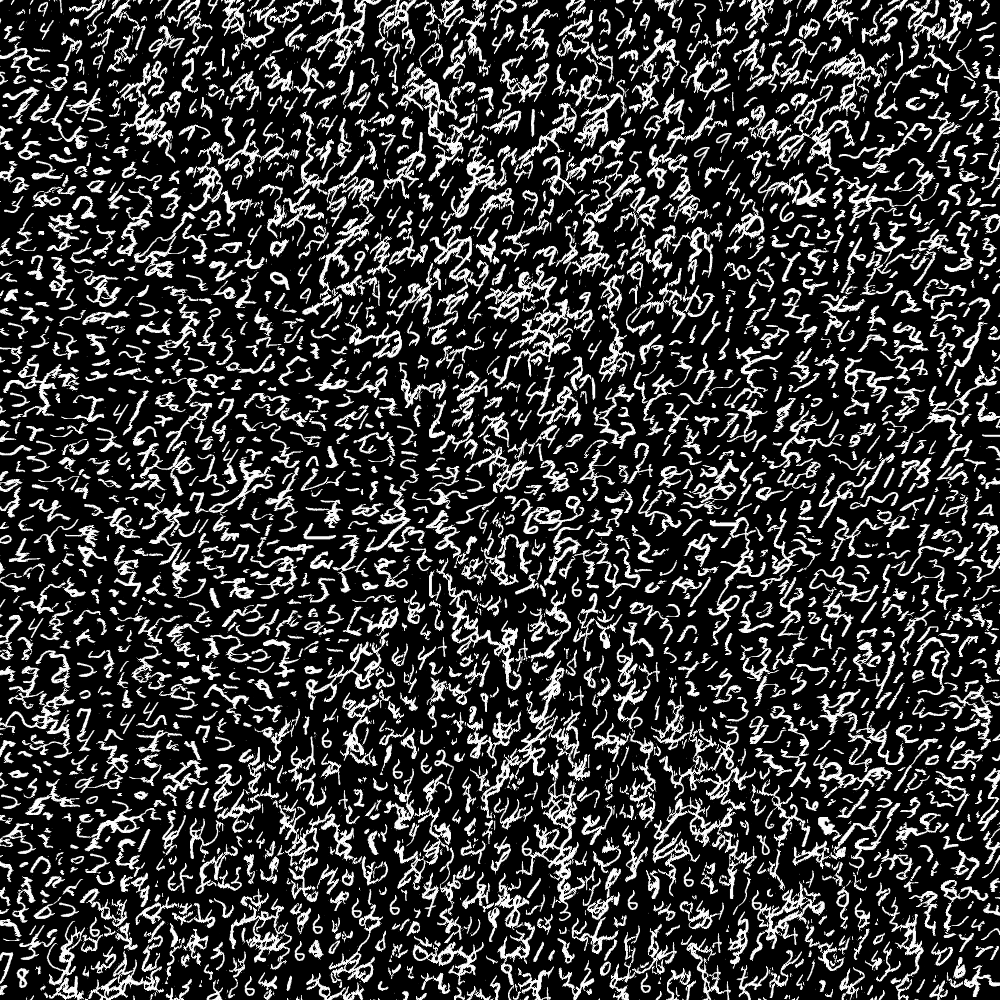
\includegraphics[width=0.7\textwidth]{../Result/mnist-patch-11.png}
        \caption{Synthesized MNIST Digits}
        \label{fig:synthesized-mnist}
    \end{subfigure}
    \caption{Synthesis of MNIST Digits}
    \label{fig:synthesis-mnist}
\end{figure}

\begin{figure}[H]
    \centering
    \begin{subfigure}[b]{0.49\textwidth}
        \centering
        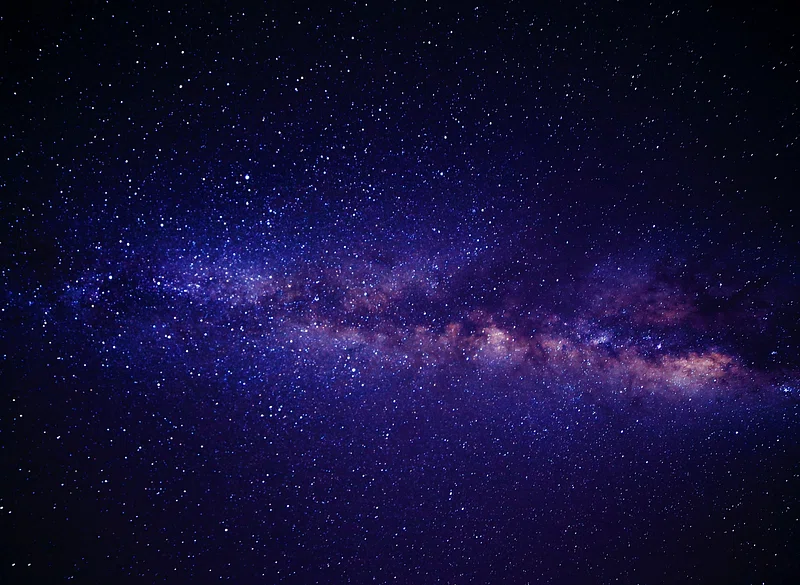
\includegraphics[width=0.6\textwidth]{../Code/Textures/galaxy.png}
        \caption{Galaxy Picture}
        \label{fig:original-galaxy}
    \end{subfigure}
    \hfill % this will add space between the subfigures
    \begin{subfigure}[b]{0.49\textwidth}
        \centering
        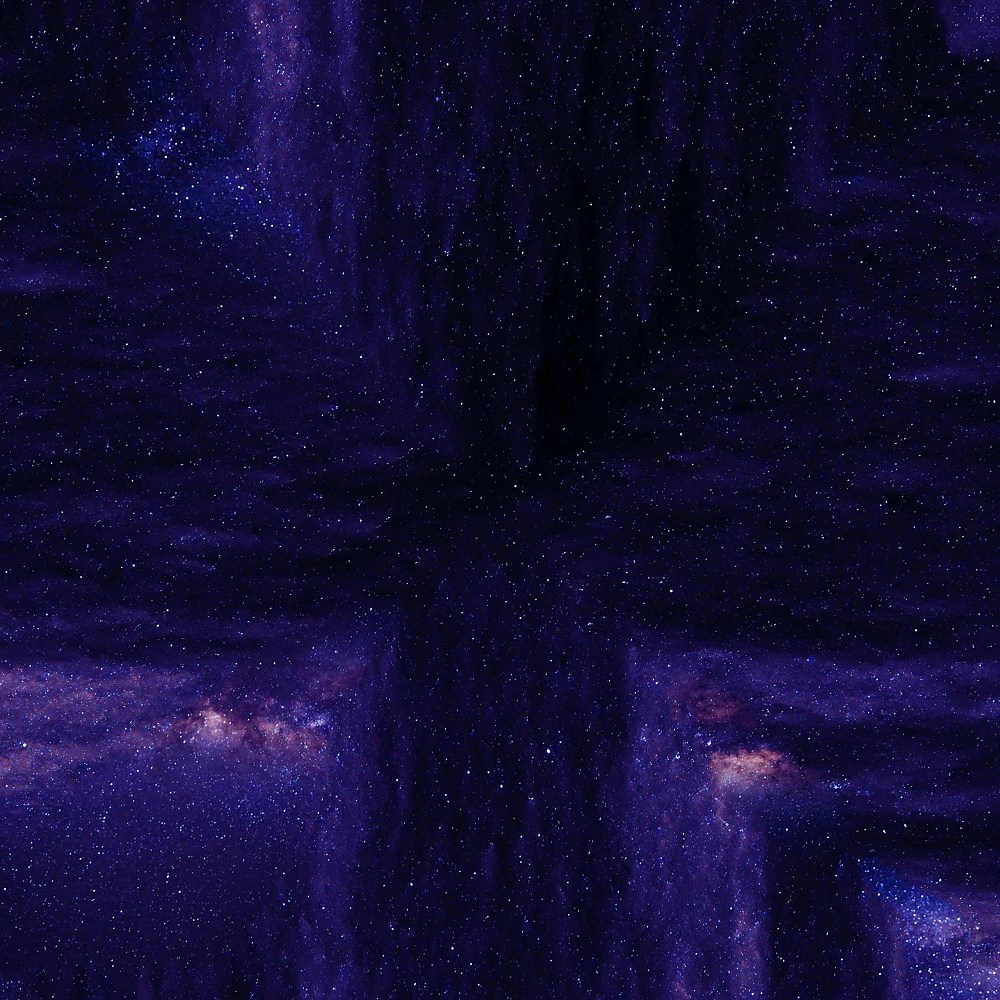
\includegraphics[width=0.7\textwidth]{../Result/galaxy.png}
        \caption{Synthesized Galaxy Picture}
        \label{fig:synthesized-galaxy}
    \end{subfigure}
    \caption{Synthesis of Galaxy Picture}
    \label{fig:synthesis-galaxy}
\end{figure}

\subsection{Different Neighborhood Patch Sizes}
In this section, we present the results of applying the non-parametric texture synthesis method on MNIST with different neighborhood sizes / patch sizes.
The results are shown in Figure~\ref{fig:mnist-diff-patch}.

\begin{figure}[H]
    \centering
    \begin{subfigure}{0.4\textwidth}
        \centering
        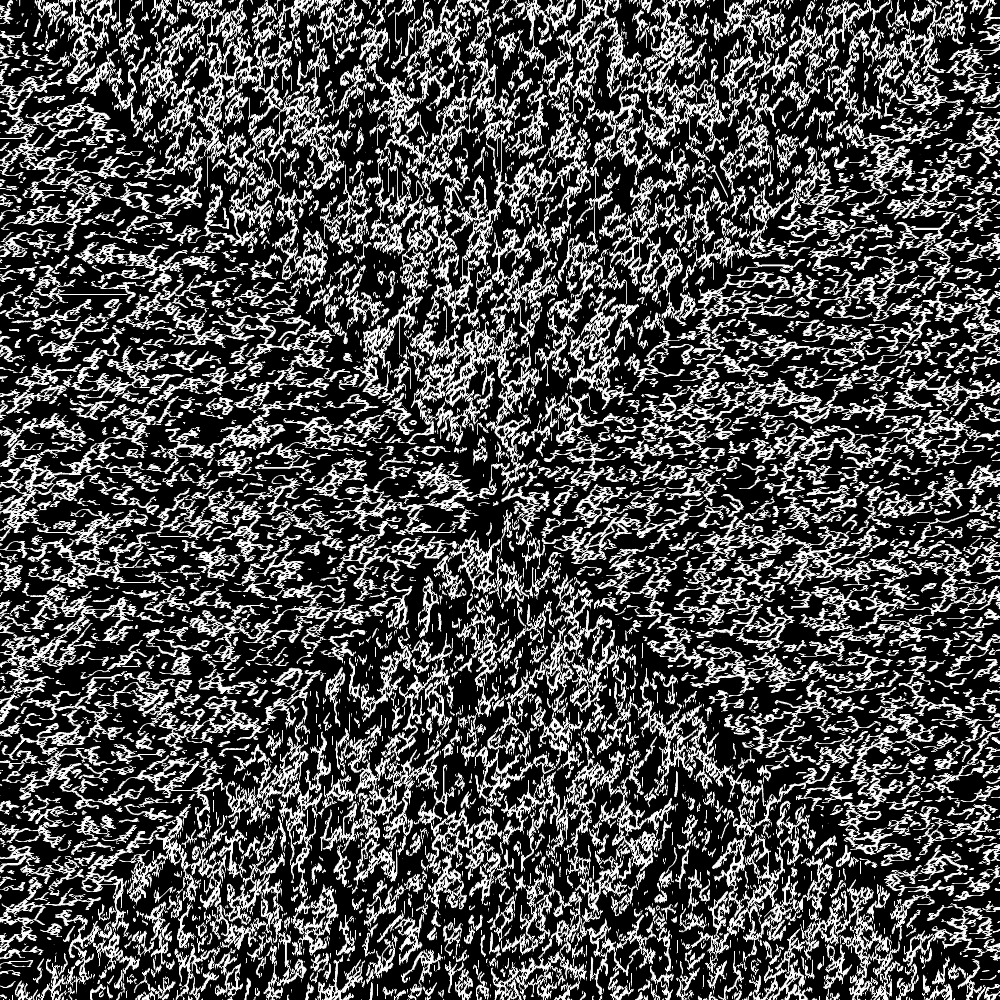
\includegraphics[width=\linewidth]{../Result/mnist-patch-5.png}
        \caption{$5 \times 5$}
        \label{fig:mnist-patch-5}
    \end{subfigure}
    \begin{subfigure}{0.4\textwidth}
        \centering
        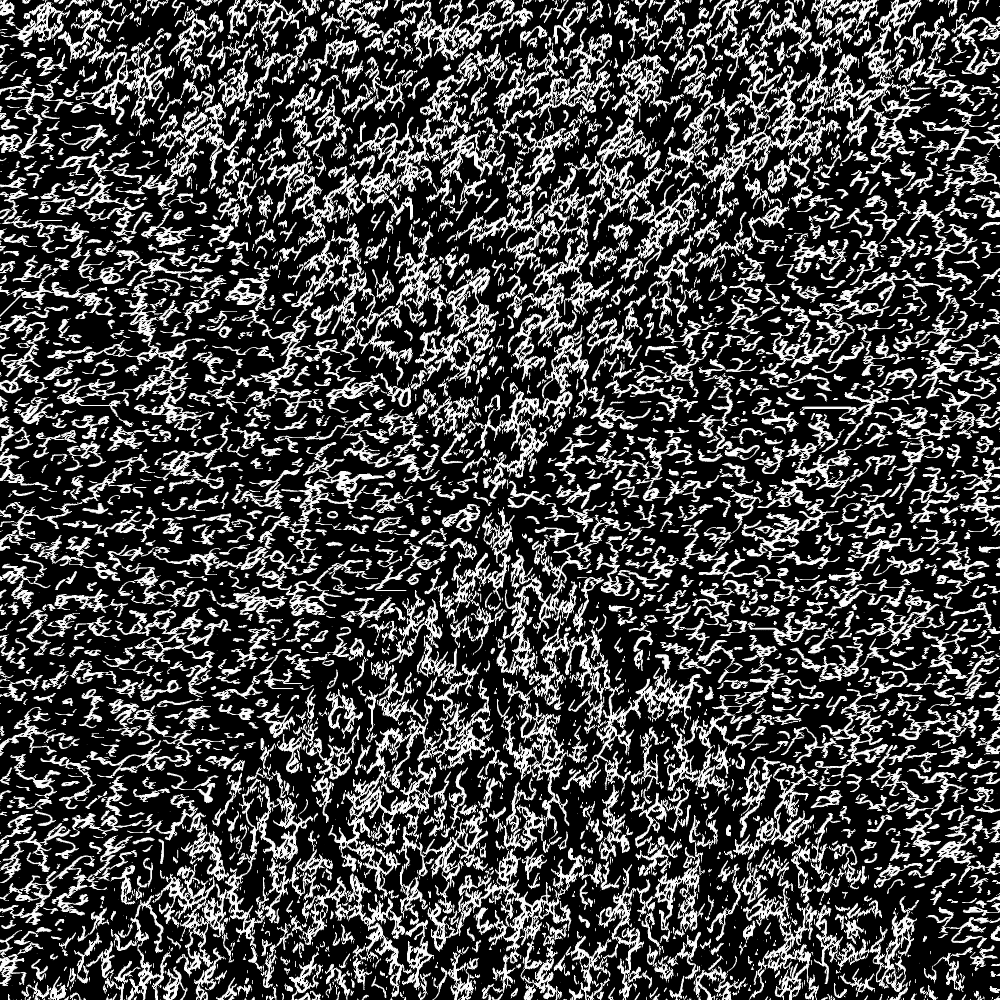
\includegraphics[width=\linewidth]{../Result/mnist-patch-7.png}
        \caption{$7 \times 7$}
        \label{fig:mnist-patch-7}
    \end{subfigure}
    \\
    \begin{subfigure}{0.4\textwidth}
        \centering
        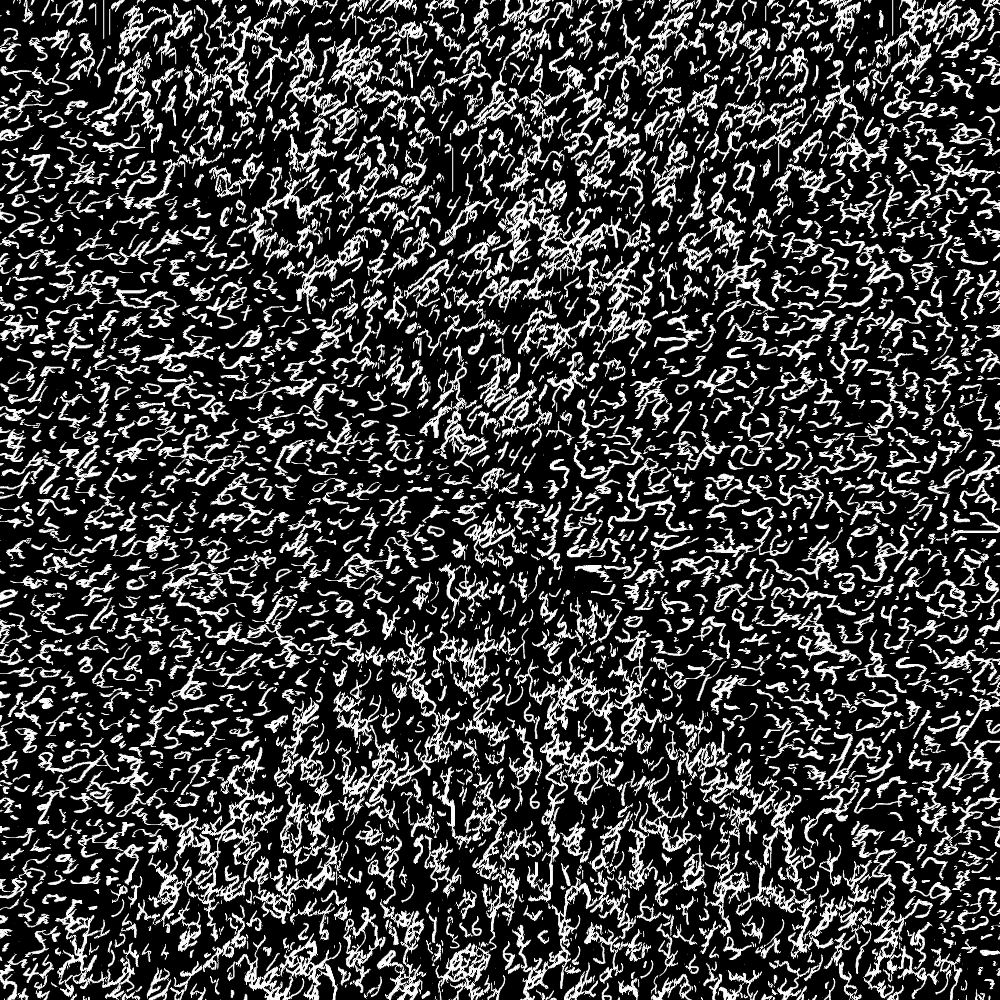
\includegraphics[width=\linewidth]{../Result/mnist-patch-9.png}
        \caption{$9 \times 9$}
        \label{fig:mnist-patch-9}
    \end{subfigure}
    \begin{subfigure}{0.4\textwidth}
        \centering
        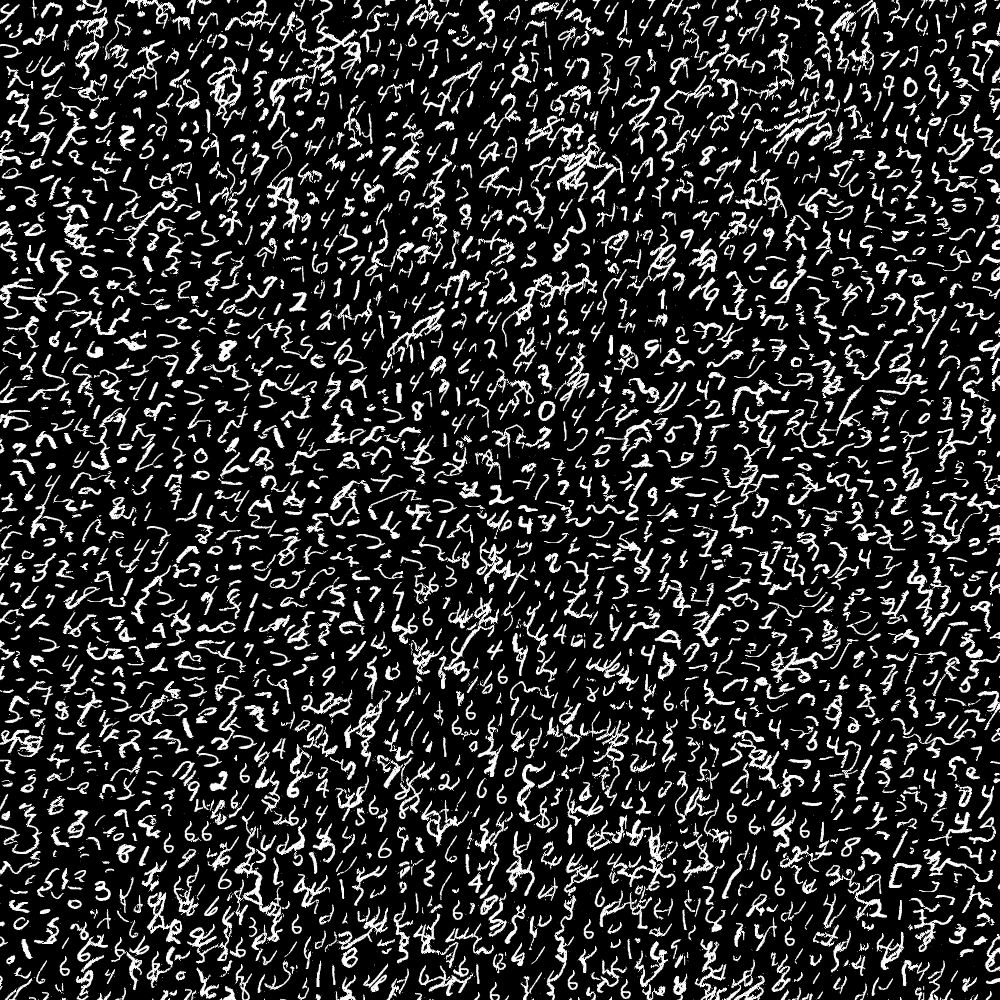
\includegraphics[width=\linewidth]{../Result/mnist-patch-15.png}
        \caption{$15 \times 15$}
        \label{fig:mnist-patch-15}
    \end{subfigure}
    \caption{Different Neighborhood Sizes for MNIST}
    \label{fig:mnist-diff-patch}
\end{figure}
As we can observe from Figure~\ref{fig:mnist-diff-patch}, when we scale the method to synthesize MNIST digits, we need to adjust the patch size to appropriately utilize the neighborhood information. In the above four cases, the patch size of $15\times 15$ produces the best synthesized result.




\printbibliography

\newpage
\section*{Appendix}
We referred to the GitHub repo: \url{https://github.com/goldbema/TextureSynthesis},
modified the code with \texttt{multiprocessing} parralelization,
and tried \texttt{PyTorch} matrix operation speedup.

\lstinputlisting[language=PythonPlus]{../Code/synthesis_fast.py}


\end{document}
